\documentclass{article}
\usepackage[margin=0.8in]{geometry} 
\usepackage{graphicx, wrapfig}
\usepackage{palatino}
\usepackage{subcaption}
\usepackage{multirow}
\usepackage{booktabs}
\begin{document}
\title{\vspace{-4ex}HW3: Unsupervised domain adaption for Statistical parsing}
\author{Rahul Huilgol (rrh2226)}
\date{}
\maketitle
\vspace{-10mm}
\section{Introduction}
Training a statistical parser requires good amount of labelled parse trees of sentences. But the parser becomes specific to the dataset it is trained on. When this parser needs to be used on data which is of a different domain than the data it is trained on, it needs to be adapted to the new domain. In this homework I study the technique of self-training for unsupervised domain adaptation. In Self-training, the parser trained on sentences from original domain called seed set, is used to label some data from the new domain to create the self-training set. It is then retrained on both seed set and self-training sets of data. The primary advantage that this technique gives us is to reduce the task of labelling sentences from all domains. In this homework, I study how well self-training works, and how it depends on size of seed set and size of self-training set.
\vspace{-2mm}
\section{Experimental setup}
The parser used for this experiment was Lexicalized Parser from Stanford NLP library. Two datasets from Penn Treebank were used, Brown and Wall Street Journal (WSJ). Brown data is composed of 8 genres. In the experiment when I consider $N$ sentences, I construct this set of $N$ sentences by choosing $N/8$ from each genre. WSJ data is composed of 24 sections. Sections 00, 01 and 24 are ignored in this homework. Whenever WSJ has been used for training and self-training, data from sections 02 to 22 were used. When WSJ was used for testing, section 23 was used.
I constructed a class DomainAdaption, which builds two LexicalizedParser objects, one called \textit{base} and other \textit{adapted}. It supports various argument options for training, adapting and testing. 
The nomenclature of in-domain and out-of-domain is such that domain refers to the domain of test set. So if the seed set is of same domain, the experiment can be called In-domain seed data.
Evaluation has been done using the metric of F-1 score, which is the harmonic mean of precision and recall.\\
\begin{wrapfigure}{r}{0.75\textwidth}
   \centering
   \hspace*{0.2in}
    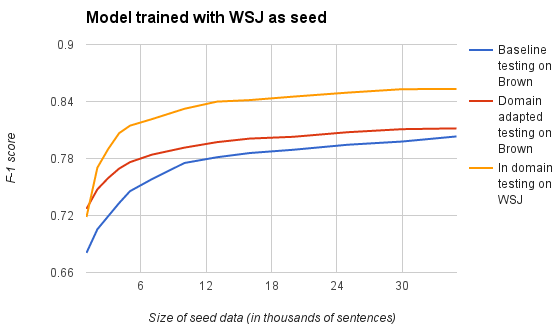
\includegraphics[width=\linewidth]{plots/q4_3.png}
    \caption{Trained with WSJ as seed, tested in domain and after adapting}
   \label{fig:q4_3}
\end{wrapfigure}
\vspace{-2mm}
\section{Results}
\subsection{WSJ as seed}
In this set of experiments, WSJ data was used as seed data to train a baseline parser. Brown data was labeled using this baseline parser to create the self-training data. This self-training data and original seed data were used to train an adapted parser. Fig.\ref{fig:q4_3} shows three curves of F-1 scores of the parser. One is the baseline parser tested in domain, second is the baseline parser tested out of domain without self-training, and third is adapted parser tested on out of domain test data. 
\clearpage
\textbf{Need for domain adaptation:} We see that scores of Baseline out-of-domain testing are significantly lower than scores of in-domain testing. This is because language especially sentence structure can vary significantly from one domain to other. WSJ only consists of news related sentences, whereas Brown consists of a diverse set of genres. The baseline parser never encountered in training the kind of sentences it sees in testing, and so does not perform as well. This shows us that there is a need to adapt a parser to the particular domain it is meant to be used. 

\begin{figure}[h]
   \centering
    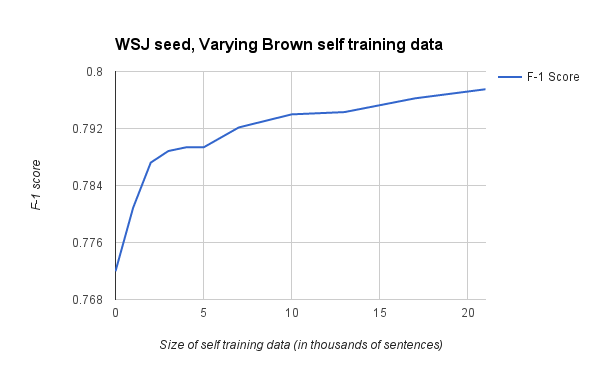
\includegraphics[width=0.75\linewidth]{plots/q5.png}
    \caption{Variation with increase of size of Brown data used for self-training}
   \label{fig:q5}
\end{figure}

\textbf{Impact of self-training:} We see here that the adapted parser gives better scores than the baseline parser when tested out of domain. This means that self-training is actually showing an improvement, because it is being trained on a diverse set of sentences and larger set of words. We can also observe that this adapted performance is quite lower than when tested in-domain. This could mean two things. Firstly, domain adaptation doesn't perform as well as building a model using labeled sentences of the same domain. This is not surprising because the labels given to self-training data by baseline parser are probably poor, because they are of different domain.  Secondly, that Brown data could be more difficult task than WSJ data. Fig.\ref{fig:q6_3} which we'll study later also indicates this because in-domain testing of Brown gives lower scores than in-domain testing of WSJ. It's also very likely that there is a combination of the two factors at play here. 

\textbf{Effect of increasing size of seed set:} We can also note that this increased performance with self-training reduces as the size of seed data increases. This is probably because more sentences in seed set captures more variation in sentence structure. This increased variation covers more variation of Brown sentences than earlier, so the F-1 scores increase.

\textbf{Effect of increasing size of self-training set:} 
Fig.\ref{fig:q5} shows how the performance of adapted parser changed as size of self-training set increases. We note that the performance is steadily increasing as size of self-training set increases, because more self-training sentences help the parser cover more variation. Despite the inaccurate labels, the self-training set has, more data makes it more likely to provide more evidence for the parser to learn better. 

\subsection{Brown as seed}
In this section, the source and target domains were flipped. Brown data was used as seed. Experiments were performed like above, to check performance of baseline parser on Brown for in-domain testing, on WSJ for out-of-domain testing without self-training, and the performance of adpated parser on out-of-domain testing. These have been summarized in Fig.\ref{fig:q6_3} and Fig.\ref{fig:q6c}. I found the following points interesting:
\begin{itemize}
  \item Brown data seems more difficult because in-domain accuracies are lower than in-domain accuracies of WSJ.
  \item Out-of-domain testing when trained with WSJ as seed and tested on Brown, gives better scores than out-of-domain testing when trained with Brown as seed and tested on WSJ. This I thought was surprising initially, because Brown is supposed to be more diverse and should cover more variety during training. But it looks like this more variety and complex diverse domains is confusing the parser and it hasn't learnt well yet. So when it is tested on WSJ, it gives a lower score than in the flipped source case.
  \begin{figure}[h]
   \centering
    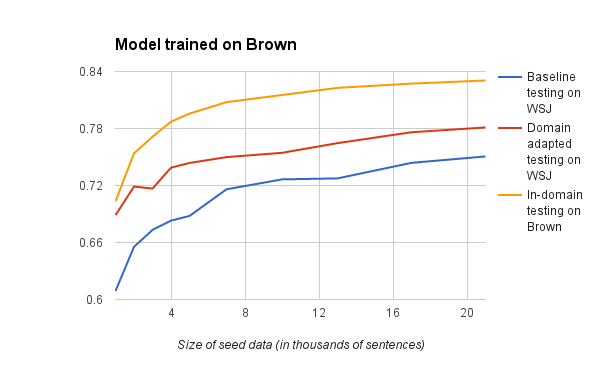
\includegraphics[width=0.75\linewidth]{plots/q6_3.png}
    \caption{Trained with Brown as seed, tested in domain and after adapting}
   \label{fig:q6_3}
\end{figure}
\begin{figure}[h]
  \vspace{-0.2in}
   \centering
    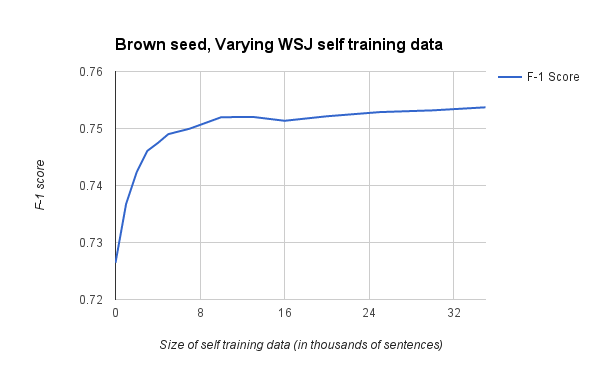
\includegraphics[width=0.75\linewidth]{plots/q6c.png}
    \caption{Variation with increase of size of WSJ data used for self-training}
   \label{fig:q6c}
\end{figure}
  \item The increase in performance due to self-training on WSJ (with Brown as seed), is higher than the increase in performance due to self-training on Brown (with WSJ as seed). This could be because Brown seed has seen some of these sentence structures but because it has to generalize over wide variety of sentences, it weighs that less. Self-training with WSJ could end up tuning the model well. Another reason could be that WSJ is an easier domain to model than Brown.
  \item Fig.\ref{fig:q6c} shows us that the increase in performance as size of self-training set increases, is slower than when size of Brown self-training data increases. I think this is because WSJ sentence structure is such that when the model is given some sentences for self-training, that is good enough to learn about the domain. But in the case of Brown, since the domain is complex, it needs more data so it can gather more examples for different sentence structures to learn.
\end{itemize}
\subsection{Comparision with Reichart and Rappoport}
My findings in general agree with their results for OI setting. Self-training substantially increased the performance in both cases despite the domains being very different. The initial increase in F-1 scores is high and the increase slows down as size of data increases.
\section{Conclusion}
Self-training proves to be a quick and easy way to adapt the domain of a parser to perform better in a new domain. Not surpisingly, this is not as good as a parser trained on the new domain itself. But in cases where labelled data is hard to find, self-training is promising, even though the improvement is only a few percentage points.
\end{document}
